\documentclass[french,10pt,twocolumn]{article}
\usepackage[T1]{fontenc}
\usepackage[utf8]{inputenc}
\usepackage{lmodern}
\usepackage[a4paper,top=0.5cm, left=0.5cm, right = 0.5cm, bottom = 0.5cm]{geometry}
\usepackage{amsmath}
\usepackage{tikz}
\usepackage{pgfplots}
\usepackage{subfigure}
\usepackage{placeins}
\usepackage{enumerate}
\usepackage{amssymb}
%\usepackage[twocolumn]{multicol}
\usepackage{titling}
%\setlength{\droptitle}{-3cm}	

\usetikzlibrary{calc}
\usetikzlibrary{decorations.markings}
\usetikzlibrary{angles,quotes} % for pic
\usetikzlibrary{arrows.meta} % for arrow size
\usetikzlibrary{bending} % for arrow head angle
\usetikzlibrary{decorations.pathmorphing} % for decorate random steps
\tikzset{>=latex} % for LaTeX arrow head

\def\spaceans{\underline{\hspace{1cm}}}
\def\spaceTF{$\big(\quad\big)$}

%\input{./styles_OMP}
\definecolor{monOrange}{RGB}{255,157,0}
\tikzset{vecteur/.style={->,thick,color=black,smooth}}
\tikzset{force/.style={->,ultra thick,rounded corners=4pt,color=monBleu,smooth,line cap=round}}
\definecolor{monBleu}{rgb}{0.2,0.4,0.6}

\title{\vspace{-1cm} \large $1^{er}$ Contrôle Continu de Mécanique du Point 2 (14/03/2024) - 	Faculté de Sciences et Technologie - UPEC \\ 	Responsable TD: Felipe FIGUEREDO ROCHA (\texttt{felipe.figueredo-rocha@u-pec.fr}) \\
	NOM:\underline{\hspace{7cm}} Prénom: \underline{\hspace{5cm}}  Numéro: \underline{\hspace{2cm}} \\
	Licence:\underline{\hspace{7cm}} Groupe: \underline{\hspace{5cm}} Note: \underline{\hspace{1.5cm}}
	\vspace{-2cm}}
\author{}
\date{}
\begin{document}
	\maketitle
	
	\vspace{-0.5cm}
	\subsection*{Rappels (regarder le tableau aussi)}
	\begin{itemize}
		\item Calculettes et téléphones \textbf{interdits}.
		\item N'oubliez vos noms en toutes les feuilles, les unités, des flèches au-dessus des vecteurs, etc.
		\item Norme produit vectoriel: |$\vec{a} \wedge \vec{b}| =  \|a\| \|b\| |\sin{\theta}(\vec{a}, \vec{b})|$.
		\item Si $(\vec{u}_x, \vec{u}_y, \vec{u}_z)$ est dite une base orthonormé direct, on a: $\vec{u}_x \wedge \vec{u}_y = \vec{u}_z$, $\vec{u}_y \wedge \vec{u}_z = \vec{u}_x$, $\vec{u}_z \wedge \vec{u}_x = \vec{u}_y$.
		\vspace{-0.5cm}
		\begin{figure}[h!]
			\centering
			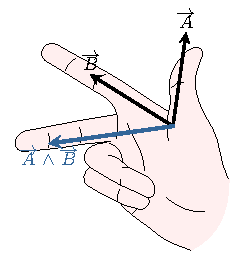
\includegraphics[width=0.3\linewidth]{regle_de_la_main_droite}
			\caption{Régle de la main droite.}
			\label{fig:regledelamaindroite}
		\end{figure}
		\vspace{-0.5cm}
		\item $(\vec{T},\vec{N},\vec{B})$, $(\vec{u}_r,\vec{u}_{\theta},\vec{u}_z)$ sont des bases orthonormés directs (dans cette l'ordre).
%		\item Repère polaire:
%		$ \begin{cases}
%			\vec{u}_r &= \cos{\theta} \Vec{u}_x + \sin{\theta} \Vec{u}_y,\\ 
%			\vec{u}_{\theta} &= -\sin{\theta} \vec{u}_x + \cos{\theta} \Vec{u}_y
%		\end{cases}
%		$ 	
		\item Repère de Frénet : $\dot{s} = \|\vec{v}\|$, $\vec{v} = \dot{s} \vec{T}$ et 
		$\vec{a} = \ddot{s} \vec{T} + \dfrac{\dot{s}^2}{R} \vec{N}$
		\item Theorème du moment cinétique :
		\begin{align*}
			\frac{d \vec{L}_0}{d t} = \sum \vec{M}_0(\vec{f}), \quad \text{où} \; \vec{L}_0 = \vec{OM}\wedge m\vec{v}, \vec{M}_0(\vec{f}) = \vec{OM}\wedge \vec{f}
		\end{align*}
	\end{itemize}
	
	\FloatBarrier
	
	\subsection*{Q1 Application du produit vectoriel dans la force électromagnétique (4pts)}
	La force électromagnétique appliqué à une particule $M$ de charge $q$, vitesse $\vec{v}$, dans un champs électrique $\vec{E}$ et champs magnétique $\vec{B}$ est donné par $\vec{f}_{EB} = q (\vec{E} + \vec{v} \wedge \vec{B})$. On pose $\vec{f}_E = q \vec{E}$, $\vec{f}_B =   q  (\vec{v} \wedge \vec{B})$, tel que $\vec{f}_{EB} = \vec{f}_E + \vec{f}_B$. On va considérer que $q$ est \textbf{négatif} et $\vec{E} = -E \vec{u}_x$, $\vec{B} = - B \vec{u}_z$, $\vec{v} = -v \vec{u}_y$, avec $E, B$ et $v$ nombres \textbf{positifs}.
	\begin{enumerate}[a)]
		\item(1,5pts) L'ensemble des vecteurs du l'ennoncé sont affichés selon le plan $Oxy$ dans la Figure \ref{fig:planOxy}, qui contient {\bf 1 (un)} erreur. Trouvez cette erreur et corrigez-le dans la Figure \ref{fig:planOxy}.  
		\item(2,5pts) Dessiner le même ensemble de vecteurs (y inclus la correction) selon le plan $Oxz$ dans la Figure \ref{fig:planOxz}.
	\end{enumerate}
	
		\vspace{-0.5cm}
	\begin{figure}[h!]
		\centering
		\subfigure[Plan $Oxy$.]{	
		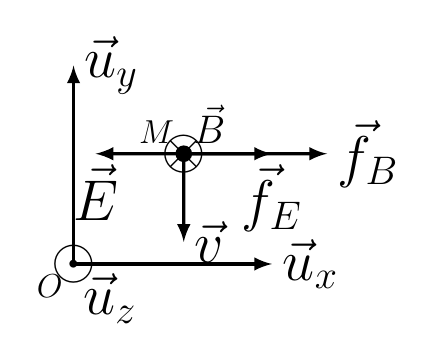
\begin{tikzpicture}[scale=1.4]
			\coordinate (O) at (0,0);
			\coordinate (X) at (1.8,0);
			\coordinate (Y) at (0,1.8);
			\coordinate (M) at (1.0, 1.0);	
			\draw[very thick,->] node[below left]{\large $O$} (O)--(X) node[right]{\huge $\vec{u}_{x}$};
			\draw[very thick,->](O)--(Y) node[right]{\huge $\vec{u}_{y}$};
			\filldraw[black] (M) circle (2pt) node[anchor=south east]{\large $M$};
			
			\draw node at (O)  {\huge $\odot$};
			\draw node[below right] at (O) {\huge $\vec{u}_z$};
			
			
			\draw[very thick,->](M)--(1.0, 0.2) node[right]{\huge $\vec{v}$};
			\draw[very thick,->](M)--(1.8, 1.0) node[below]{\huge $\vec{f}_E$};
			\draw[very thick,->](M)--(0.2, 1.0) node[below]{\huge $\vec{E}$};
			\draw[very thick,->](M)--(2.3, 1.0) node[right]{\huge $\vec{f}_B$};
			
			\draw node at (M)  {\huge $\otimes$};
			\draw node[above right] at (M) {\Large $\vec{B}$};
			
		\end{tikzpicture}
		\label{fig:planOxy}
		}
		\subfigure[Plan $Oxz$.]{
		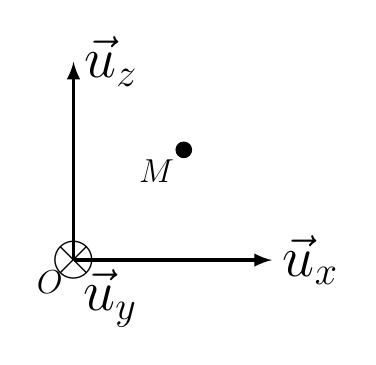
\begin{tikzpicture}[scale=1.4]
			\coordinate (O) at (0,0);
			\coordinate (X) at (1.8,0);
			\coordinate (Y) at (0,1.8);
			\coordinate (M) at (1.0, 1.0);	
			\draw[very thick,->] node[below left]{\large $O$} (O)--(X) node[right]{\huge $\vec{u}_{x}$};
			\draw[very thick,->](O)--(Y) node[right]{\huge $\vec{u}_{z}$};
			\filldraw[black] (M) circle (2pt) node[anchor=north east]{\large $M$};
			
			\draw node at (O)  {\huge $\otimes$};
			\draw node[below right] at (O) {\huge $\vec{u}_y$};
		\end{tikzpicture}
		\label{fig:planOxz}
		}
		\caption{Q2}
		\label{fig:q2}
	\end{figure}
	\vspace{-1cm}	
	\FloatBarrier
	
	\subsection*{Q2 : Un esquimau tombé dans un trou (8pts)} 
	Un enfant esquimau tombe dans un trou sur la neige quand il jouait avec ses amis aux alentours de l'extremité gauche du trou. Ce trou a le format d'une demi-sphère de rayon $R$ et de centre $O$. Il va glisser vers le fond du trou avec un frottement $\vec{f}$ (avec sa norme noté par $f$). La position de l'enfant, assimilé à un point matériel $M$ de masse $m$ est repérée par l’angle $\theta$ par rapport à $\vec{u}_x$ (augmentant vers la direction de $\vec{u}_y$). La norme de l'accéleration de la pesanteur est dénoté $g$, tel $\vec{g} = g\vec{u}_x$ pointe vers le bas. L'objectif de cet exercice est d'étudier le mouvement en repère de \textbf{Frénet}. 
	\begin{enumerate}[a)]
		\item(1,5pt) Complétez la figure ci-dessous en plaçant $\vec{T}$ (\textbf{supposant $\dot{\theta}<0$}) et $\vec{N}$.
		\begin{figure}[h!]
			\centering
			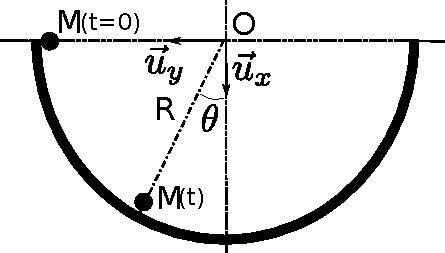
\includegraphics[width=0.5\linewidth]{trou}
		\end{figure}
		\item(1,5pt) Donner les expressions de toutes les forces en repère de Frénet.
		\item(2,0pt) Appliquer le principe fondamentale de la dynamique (PFD) en repère de Frénet.
		\item(1,0pt) Expliciter $\theta(t=0)$ et $\dot{s}(t=0)$.
		\item(2,0pt) On va supposer que $f = \alpha R_N$ ($\alpha >0$ un coefficient donné). Pour l'instant initial, déterminer $R_N(t=0), f(t=0)$ et $\ddot{s}(t=0)$ en utilisant les deux équations différentielles trouvés dans le PFD.
	\end{enumerate}

	\subsection*{Q3 : Le modèle de Bohr (8pts)}	
	Le modèle de Bohr représente l’atome d’hydrogène constitué par un proton ponctuel de charge $q$ et de masse $m_P$ autour duquel gravite, en orbite circulaire, un électron de charge $-q$ et de masse $m_e$. On note $O$ le centre de l’orbite (le proton), $M$ la position du électron, $R$ son rayon et $v$ la norme de la vitesse orbitale (tangentielle au cercle). On néglige toutes les forces, sauf la force de Coulomb de norme $F =  \dfrac{q^2}{4\pi\varepsilon_0 R^2}$ (obs1: le vecteur $\vec{F}$ sera défini en fonction du repère choisi, obs2: $\varepsilon_0$ est une constante).
	\begin{enumerate}[a)]
	\item (2 pts) Dessiner un schèma du problème avec les éléments décrits ci-dessus, y inclus le vecteur $\vec{F}$ agissant sur l'électron. Répresenter aussi les vecteurs de base repère (cylindrique ou de Frénet selon votre préférence).
	\item (1,5pt) Ecrire les vecteurs $\vec{OM}$, $\vec{v}$ et $\vec{F}$ dans la base choisi.
	\item (1,5pts) Montrer que $\vec{M}_0(\vec{F}) = \vec{0}$.
	\item (1,5pts) Le moment cinétique $\vec{L}_0$ du électron sera-t-il conservé?  justifier votre réponse en utilisant le theorème du moment cinétique.
	\item (1,5pt) Calculer $\vec{L}_0$.
	\end{enumerate}

\end{document}
